\subsection*{Lösungen zu Kapitel~\ref{kapitel:SechsInkreise}: \emph{Das Sechs-Inkreise-Lemma}}

\begin{proof}[Lösung zu Aufgabe~\ref{aufgabe:SechsInkreiseSehnenviereck}]
	Die Inkreise von $DAP$ und $BCP$ haben zwei gemeinsame äußere Tangenten. Eine davon ist offenbar $CD$; die andere bezeichnen wir mit $t$. Indem wir das Sechs-Inkreise-Lemma in dem Fall anwenden, dass $\omega_A$ und $\omega_B$ zu Punkten degeneriert sind und außerdem $C_D$ und $D_C$ im Punkt $P$ zusammenfallen, erhalten wir sofort, dass $t$ auch eine Tangente an den Inkreis von $ABP$ ist.	
	\begin{figure}[ht]
		\centering
		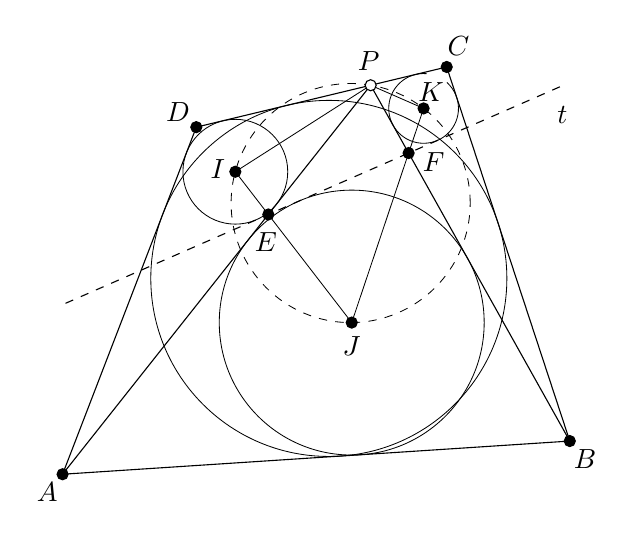
\begin{tikzpicture}[x=0.85cm,y=0.85cm]
			\draw [line width=0.3] (-10.79,11.71) circle (2.66);
			\draw [line width=0.3] (-12.187,13.304) coordinate (I) circle (0.783);
			\draw [line width=0.3] (-10.448,11.05) coordinate (J) circle (1.979);
			\coordinate (K) at (-9.374,14.25);
			\draw [line width=0.3,shift={(K)}] (85:0.521) arc (85:408:0.521);
			\draw [dashed,line width=0.3] (-10.464,12.836) circle (1.786);
			\coordinate (A) at (-14.768,8.784);
			\coordinate (B) at (-7.19,9.28);
			\coordinate (C) at (-9.029,14.869);
			\coordinate (D) at (-12.77,13.97);
			\coordinate (E) at (-11.694,12.665);
			\coordinate (F) at (-9.598,13.583);
			\coordinate (P) at (-10.165,14.596);
			\draw (A) to (B) to (C) to (D) to cycle;
			\draw (A) to (P) to (B);
			%\draw [line width=0.3] (B) to (I) to (D);
			\draw [shorten <=-8em,shorten >=-6em, dashed] (E) to (F);
			\draw [line width=0.3] (P) to (I) to (J) to (K) to cycle;
			\draw[fill=black] (A) circle (2pt) node[shift={(230:2ex)}] {$A$};
			\draw[fill=black] (B) circle (2pt) node[shift={(310:2ex)}] {$B$};
			\draw[fill=black] (C) circle (2pt) node[shift={(60:2ex)}] {$C$};
			\draw[fill=black] (D) circle (2pt) node[shift={(140:2ex)}] {$D$};
			\draw[fill=black] (E) circle (2pt) node[shift={(265:2.35ex)}] {$E$};
			\draw[fill=black] (F) circle (2pt) node[shift={(340:2.25ex)}] {$F$};
			\draw[fill=black] (I) circle (2pt) node[shift={(170:1.5ex)}] {$I$};
			\draw[fill=black] (J) circle (2pt) node[shift={(270:2ex)}] {$J$};
			\draw[fill=black] (K) circle (2pt) node[shift={(65:1.5ex)}] {$K$};
			\draw[fill=white] (P) circle (2pt) node[shift={(95:2ex)}] {$P$};
			\node at (-7.3,14.15) {$t$};
		\end{tikzpicture}
	\end{figure}
	
	Seien $E$ und $F$ die Schnittpunkte von $t$ mit $AP$ und $BP$ (in der Notation des Sechs-Inkreise-Lemmas wären das die Punkte $B_D$ und $A_C$). Nachdem $t$ nun auch eine Tangente an den Inkreis von $ABP$ ist, liegen $I$, $J$ und $E$ auf der Winkelhalbierenden von $\winkel(AP,t)$. Analog liegen $J$, $K$ und $F$ auf der Winkelhalbierenden von $\winkel(t,BP)$. Also erhalten wir die Gleichung $\winkel KJI=180^\circ-\winkel EFJ-\winkel JEF=180^\circ-\winkel PEI-\winkel KFP$. Andererseits gilt aber auch $\winkel IPK=180^\circ-\winkel DPI-\winkel KPC=180^\circ-\winkel IPE-\winkel FPK$. Nach den obigen Gleichungen und wegen der Innenwinkelsumme in $EPI$ und $FKP$ gilt nun
	\begin{align*}
		\winkel KJI+\winkel IPK&=360^\circ-\winkel PEI-\winkel IPE-\winkel KFP-\winkel FPK\,,\\
		\winkel JIP+\winkel PKJ&=360^\circ-\winkel PEI-\winkel IPE-\winkel KFP-\winkel FPK\,.
	\end{align*}
	Folglich $\winkel KJI+\winkel IPK=\winkel JIP+\winkel PKJ$. Dann muss aber $\winkel KJI+\winkel IPK=180^\circ$ sein, weshalb $PIJK$ in der Tat ein Sehnenviereck ist.
\end{proof}

\begin{proof}[Lösung zu Aufgabe~\ref{aufgabe:531246} \textmd{(\href{https://www.mathematik-olympiaden.de/moev/index.php?option=com_download&thema=a&datei=A53124b.pdf&format=raw}{MO 531246})}]
	Weil $P$ auf der Winkelhalbierenden $AI$ von $\winkel BAD$ liegt, gibt es einen Kreis $\omega_A$ mit Mittelpunkt $P$, der $\overline{AB}$ und $\overline{DA}$ berührt. Analog gibt es einen Kreis $\omega_C$ mit Mittelpunkt $Q$, der $\overline{BC}$ und $\overline{CD}$ berührt.
	\begin{figure}[ht]
		\centering
		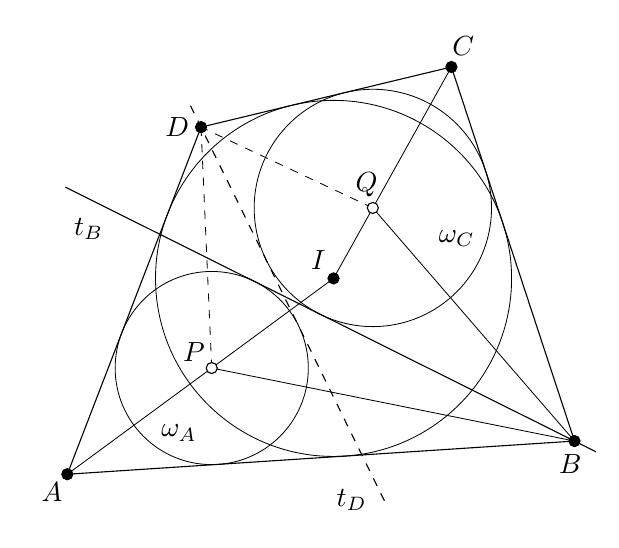
\begin{tikzpicture}[x=0.85cm,y=0.85cm]
			\draw [line width=0.3] (-10.79,11.71) coordinate (I) circle (2.66);
			\draw [line width=0.3] (-12.61,10.371) coordinate (P) circle (1.443);
			\draw [line width=0.3] (-10.203,12.763) coordinate (Q) circle (1.773);
			\coordinate (A) at (-14.768,8.784);
			\coordinate (B) at (-7.19,9.28);
			\coordinate (C) at (-9.029,14.869);
			\coordinate (D) at (-12.77,13.97);
			\draw (A) to (B) to (C) to (D) to cycle;
			\draw [line width=0.3] (A) to (I) to (C);
			%\draw [line width=0.3] (B) to (I) to (D);
			\draw [shorten <=-2ex,shorten >=-2em, dashed] (D) to (-10.366,9.072);
			\draw [shorten <=-2ex,shorten >=1.5em] (B) to (-15.352,13.35);
			\draw [line width=0.3] (P) to (B) to (Q);
			\draw [dashed,line width=0.3] (P) to (D);
			\draw [dashed,line width=0.3] (Q) to (D);
			%\draw [shift={(B)}, line width=0.3] (108.215:0.52cm) arc (108.215:130.856:0.52cm);
			%\draw [shift={(B)}, line width=0.3] (130.856:0.57cm) arc (130.856:153.497:0.57cm);
			%\draw [shift={(B)}, line width=0.3] (153.497:0.52cm) arc (153.497:168.622:0.52cm);
			%\draw [shift={(B)}, line width=0.3] (153.497:0.47cm) arc (153.497:168.622:0.47cm);
			%\draw [shift={(B)}, line width=0.3] (168.622:0.57cm) arc (168.622:183.746:0.57cm);
			%\draw [shift={(B)}, line width=0.3] (168.622:0.62cm) arc (168.622:183.746:0.62cm);
			\draw[fill=black] (A) circle (2pt) node[shift={(230:2ex)}] {$A$};
			\draw[fill=black] (B) circle (2pt) node[shift={(260:2ex)}] {$B$};
			\draw[fill=black] (C) circle (2pt) node[shift={(60:2ex)}] {$C$};
			\draw[fill=black] (D) circle (2pt) node[shift={(180:2ex)}] {$D$};
			\draw[fill=black] (I) circle (2pt) node[shift={(130:2ex)}] {$I$};
			\draw[fill=white] (P) circle (2pt) node[shift={(138:2ex)}] {$P$};
			\draw[fill=white] (Q) circle (2pt) node[shift={(105:2ex)}] {$Q$};
			\node at (-13.1,9.4) {$\omega_A$};
			\node at (-8.95,12.3) {$\omega_C$};
			\node at (-14.45,12.45) {$t_B$};
			\node at (-10.52,8.4) {$t_D$};
		\end{tikzpicture}
	\end{figure}
	
	Sei nun $t_B$ die von $AB$ verschiedene Tangente durch $B$ an $\omega_A$. Dann ist $BP$ die Winkelhalbierende von $\winkel (t_B,AB)$. Analog sei $t_B'$ die von $BC$ verschiedene Tangente durch $B$ an $\omega_C$, sodass $BQ$ die Winkelhalbierende von $\winkel (BC,t_B')$ ist. Die Voraussetzung $\winkel QBP=\frac12\winkel CBA$ sagt uns nun genau, dass $t_B=t_B'$ gelten muss. Mit anderen Worten: Die Tangente $t_B$ an $\omega_A$ ist auch eine Tangente an den Kreis $\omega_C$.
	
	Mit einem völlig analogen Argument sehen wir: Um $\winkel PDQ=\frac12\winkel ADC$ zu beweisen, müssen wir nur zeigen, dass die von $DA$ verschiedene Tangente $t_D$ durch $D$ an $\omega_A$ auch eine Tangente an $\omega_C$ ist. Das folgt aber direkt aus dem Sechs-Inkreise-Lemma in dem Spezialfall, dass die Kreise $\omega_B$, $\omega_D$ und $\omega$ zu Punkten degeneriert sind.
\end{proof}